\begin{frame}
	\frametitle{Outline}
	\begin{itemize}
		\item % TODO
	\end{itemize}
\end{frame}

\begin{frame}
	\frametitle{Experiments 1 \& 2: Hyperparameter Tuning}

	\includegraphics[height=95pt]{exp1_slice0}\hfill%
	\includegraphics[height=95pt]{exp1_slice1}\hfill%
	\includegraphics[height=95pt]{exp1_slice2}

	\begin{columns}
		\column{0.28\textwidth}
		\includegraphics[height=95pt]{exp2_time_vs_reg}

		\column{0.72\textwidth}
		\begin{itemize}
			\item
				Experiment 1 ($3\times$ top), Experiment 2 (left).
				Plots show $\overline{t}_\text{pred.}$ vs.~$R^2$ (best = upper
				left).
			\item
				Showing the best 20 surrogates per family.
			\item
				Omitting discrete features yields only a negligible
				improvement in performance.
			\item
				Overall dominated by tree-based surrogates (GBTs, ERTs) and
				neural networks.
		\end{itemize}
	\end{columns}

\end{frame}

\begin{frame}
	\frametitle{Experiment 3: Scaling Benchmark}
	\begin{columns}
		\column{0.5\textwidth}
		\begin{itemize}
			\item
				We observe a hierarchy.
			\item
				Best-performing families from the previous experiments also scale the
				best in $t_\text{pred}$.
			\item
				More samples: neural networks outperform tree-based models.
		\end{itemize}

		\column{0.5\textwidth}
		\begin{itemize}
			\item
				Instance-based surrogates offer train trivially but have
				complex lookup strategies.
			\item
				Neural networks show inverse scaling due to
				parallelization.
		\end{itemize}
	\end{columns}

	\vspace{1em}

	\includegraphics[height=95pt]{scaling_metric_r2}
	\includegraphics[height=95pt]{scaling_time_train}
	\includegraphics[height=95pt]{scaling_time_pred}
\end{frame}

\begin{frame}
	\frametitle{Experiment 4: Model Comparison}
	\begin{columns}
		\column{0.59\textwidth}
		\begin{itemize}
			\item
				Plots show true vs.~predicted TBR by Models~1-8,
				coloured by density.
			\item
				Best regression performance:
				\begin{itemize}
					\item
						Model 1, ANN, 500K~samples.
					\item
						$R^2=\num{0.998}$,
						$\sigma=\num{0.013}$,
					\item
						$\overline{t}_{\text{pred.}}=\SI{1.124}{\micro\second}$,
						$\num{6916416} \times$~faster.
				\end{itemize}
			\item
				Fastest prediction:\textsuperscript{\textdagger}
				\begin{itemize}
					\item
						Model 2, ANN, 500K~samples.
					\item
						$R^2=\num{0.985}$,
						$\sigma=\num{0.033}$,
					\item
						$\overline{t}_{\text{pred.}}=\SI{0.898}{\micro\second}$,
						$\num{8659251} \times$~faster.
				\end{itemize}
			\item
				Smallest training set:\textsuperscript{\textdagger}
				\begin{itemize}
					\item
						Model 4, GBT, 10K~samples.
					\item
						$R^2=\num{0.913}$,
						$\sigma=\num{0.072}$,
					\item
						$\overline{t}_{\text{pred.}}=\SI{6.125}{\micro\second}$,
						$\num{1269777} \times$~faster.
				\end{itemize}
		\end{itemize}

		{\footnotesize
			\textsuperscript{\textdagger}
			with acceptable regression performance.
		}

		\column{0.41\textwidth}
		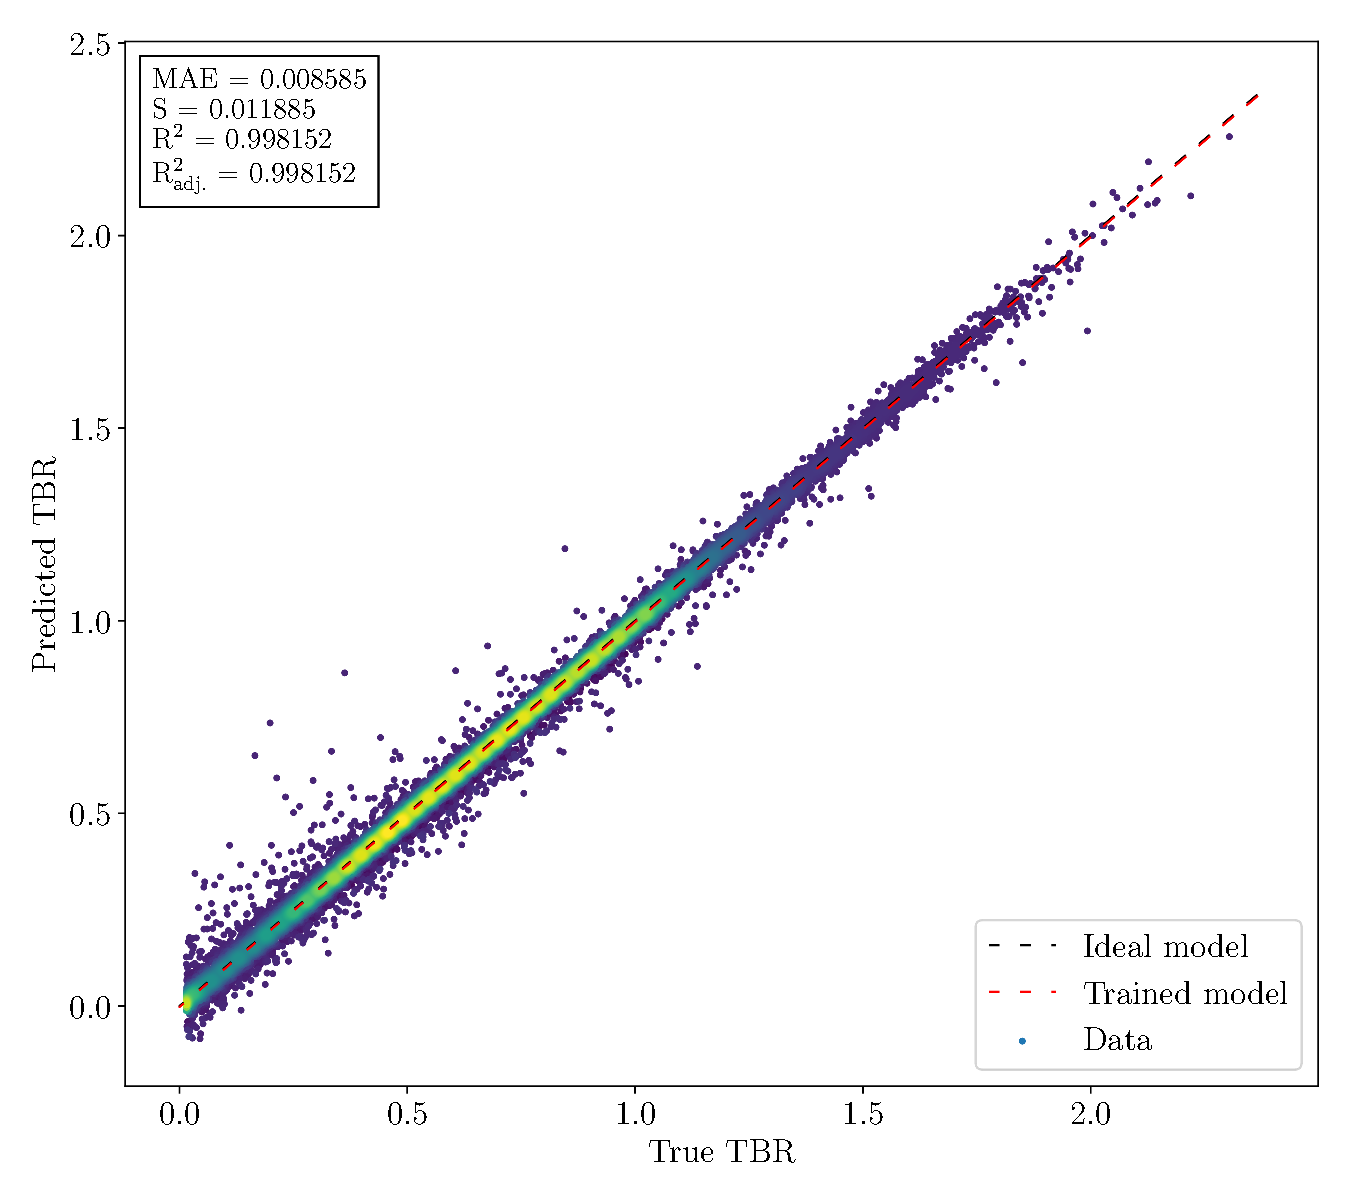
\includegraphics[height=60pt]{exp4_model6_rasterized}\hfill%
		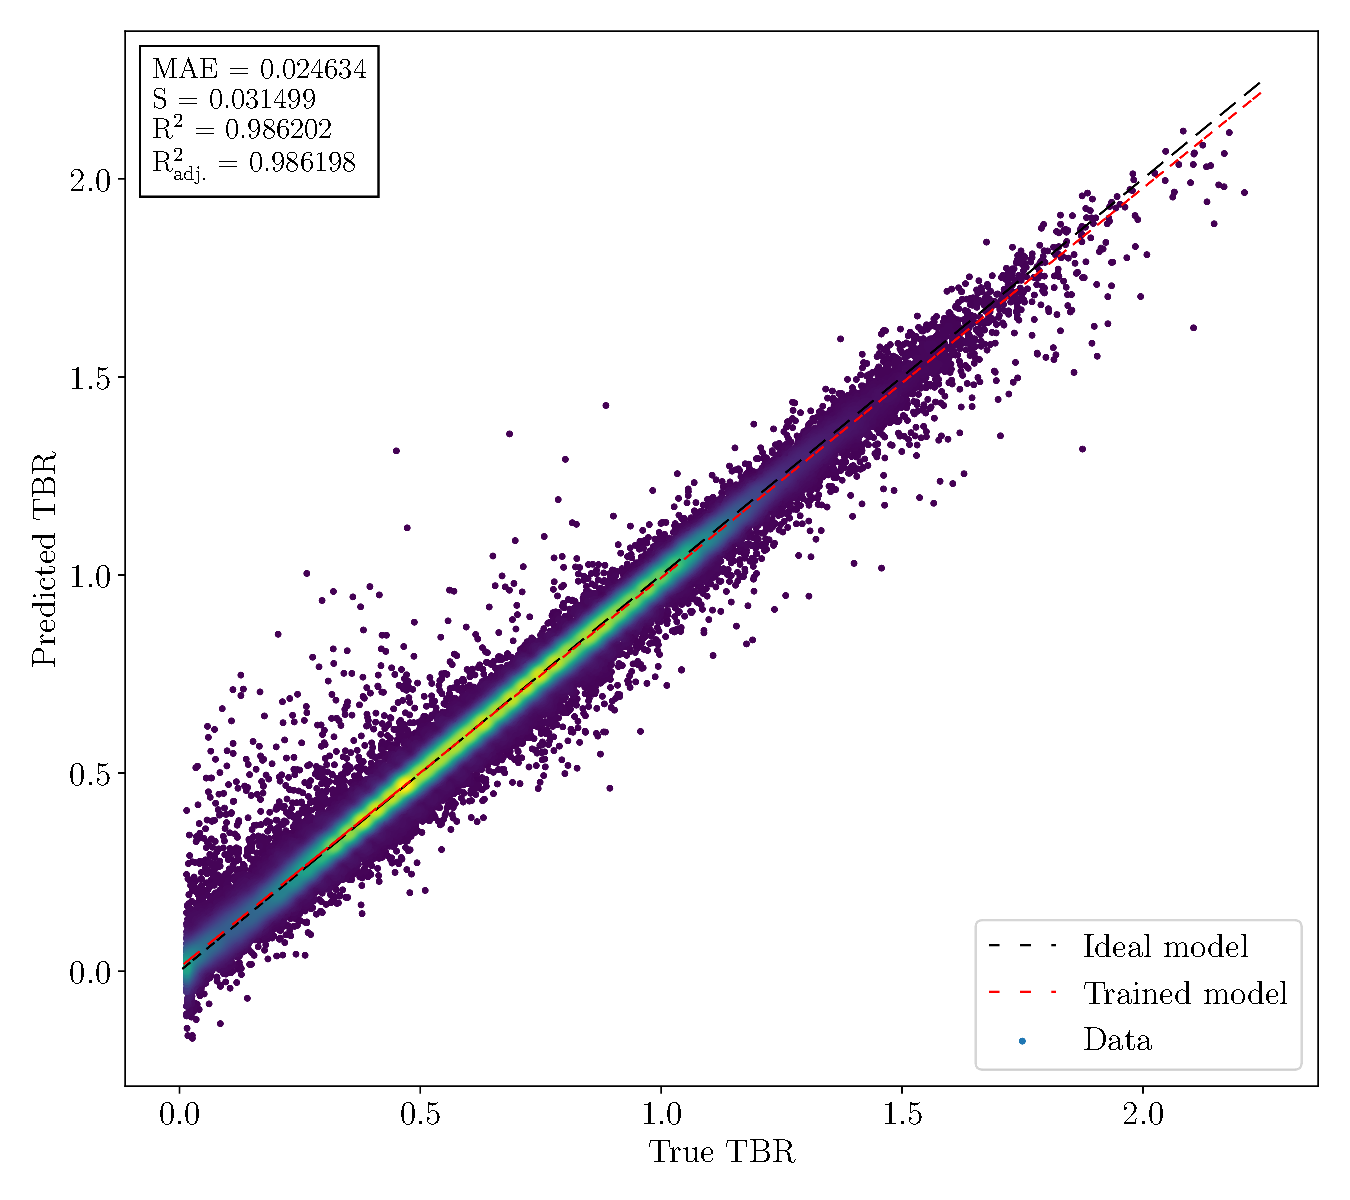
\includegraphics[height=60pt]{exp4_model7_rasterized}\\\vspace{-4pt}%
		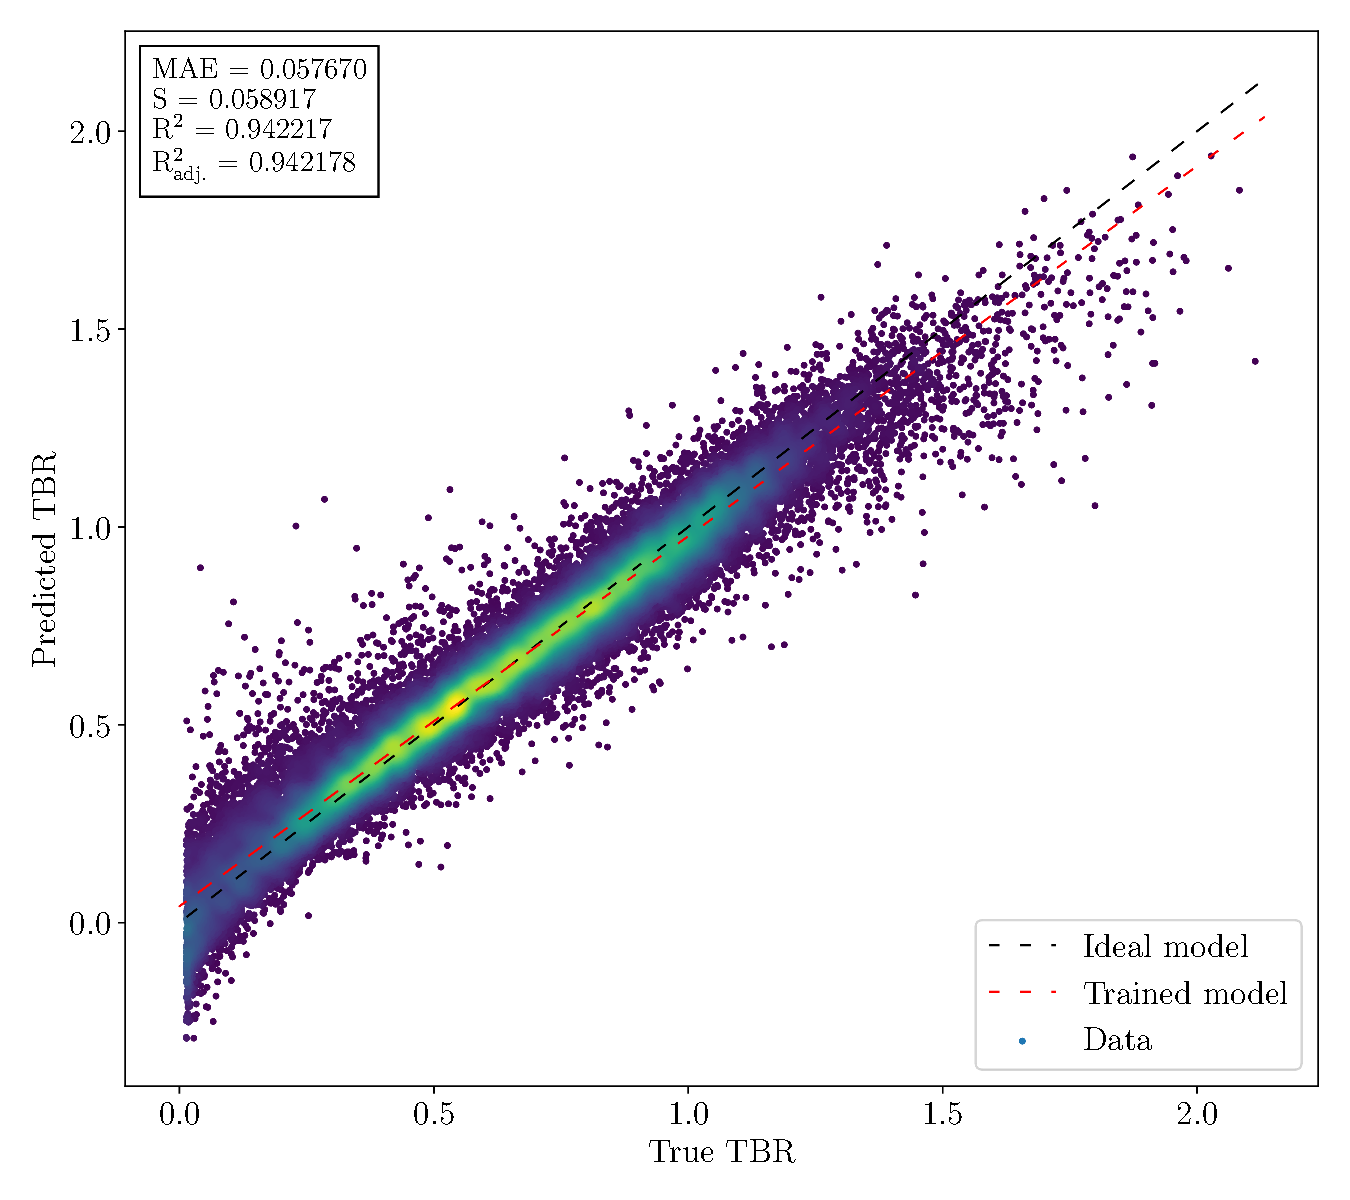
\includegraphics[height=60pt]{exp4_model1_rasterized}\hfill%
		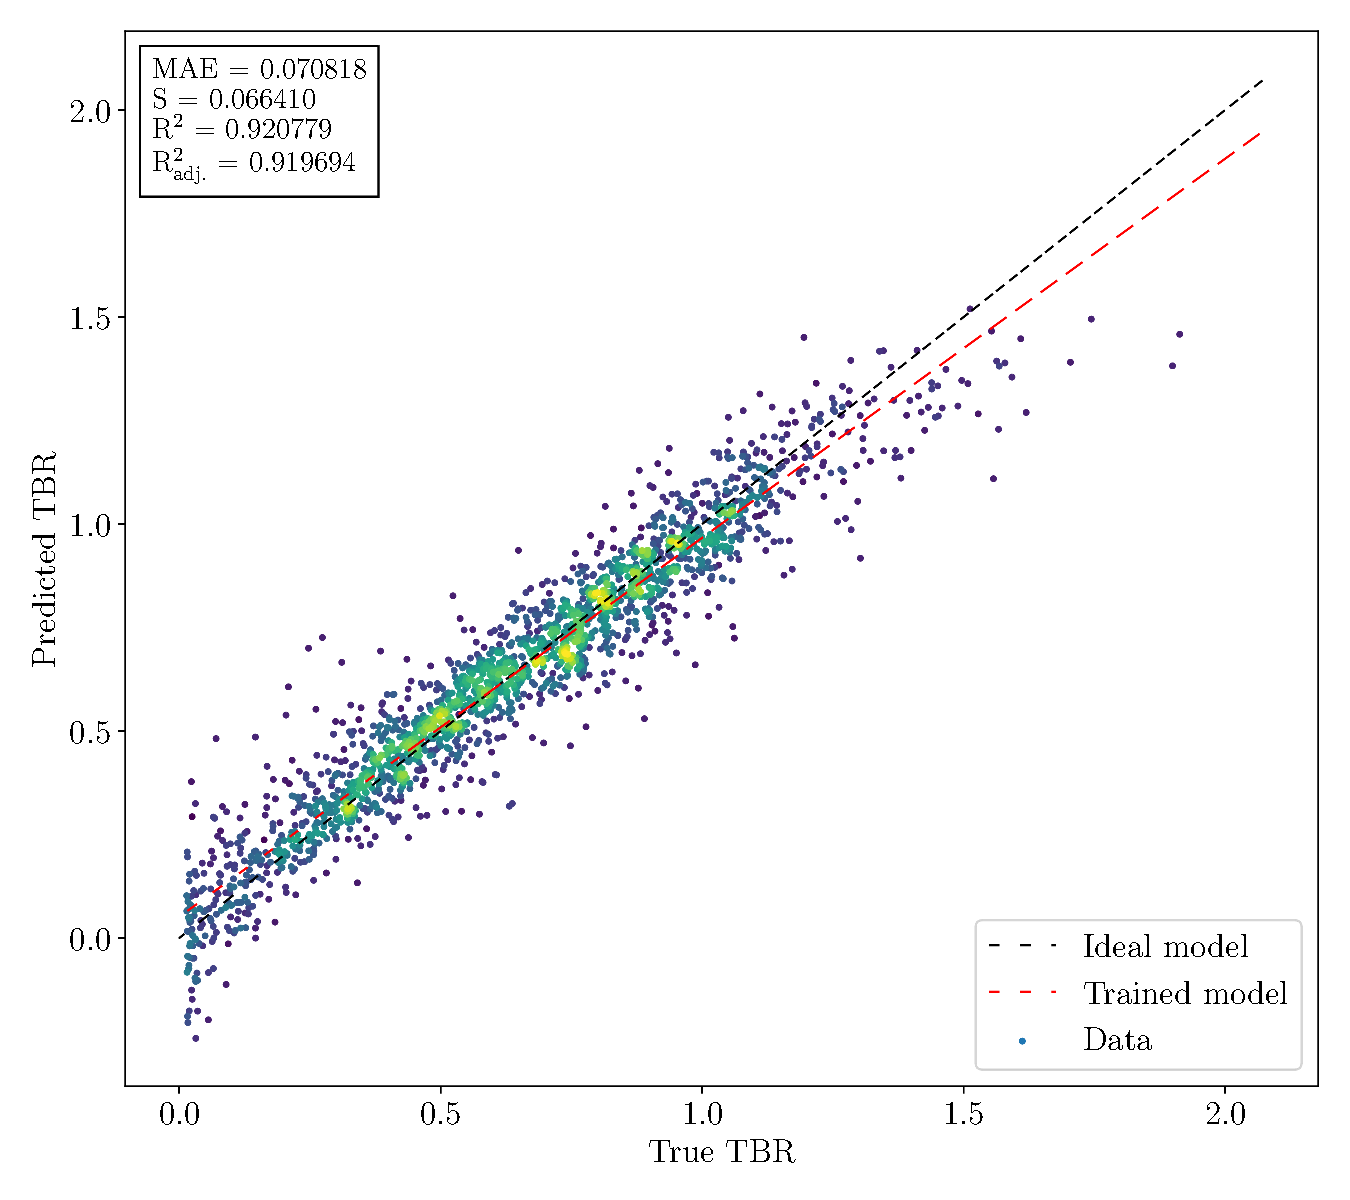
\includegraphics[height=60pt]{exp4_model3_rasterized}\\\vspace{-4pt}%
		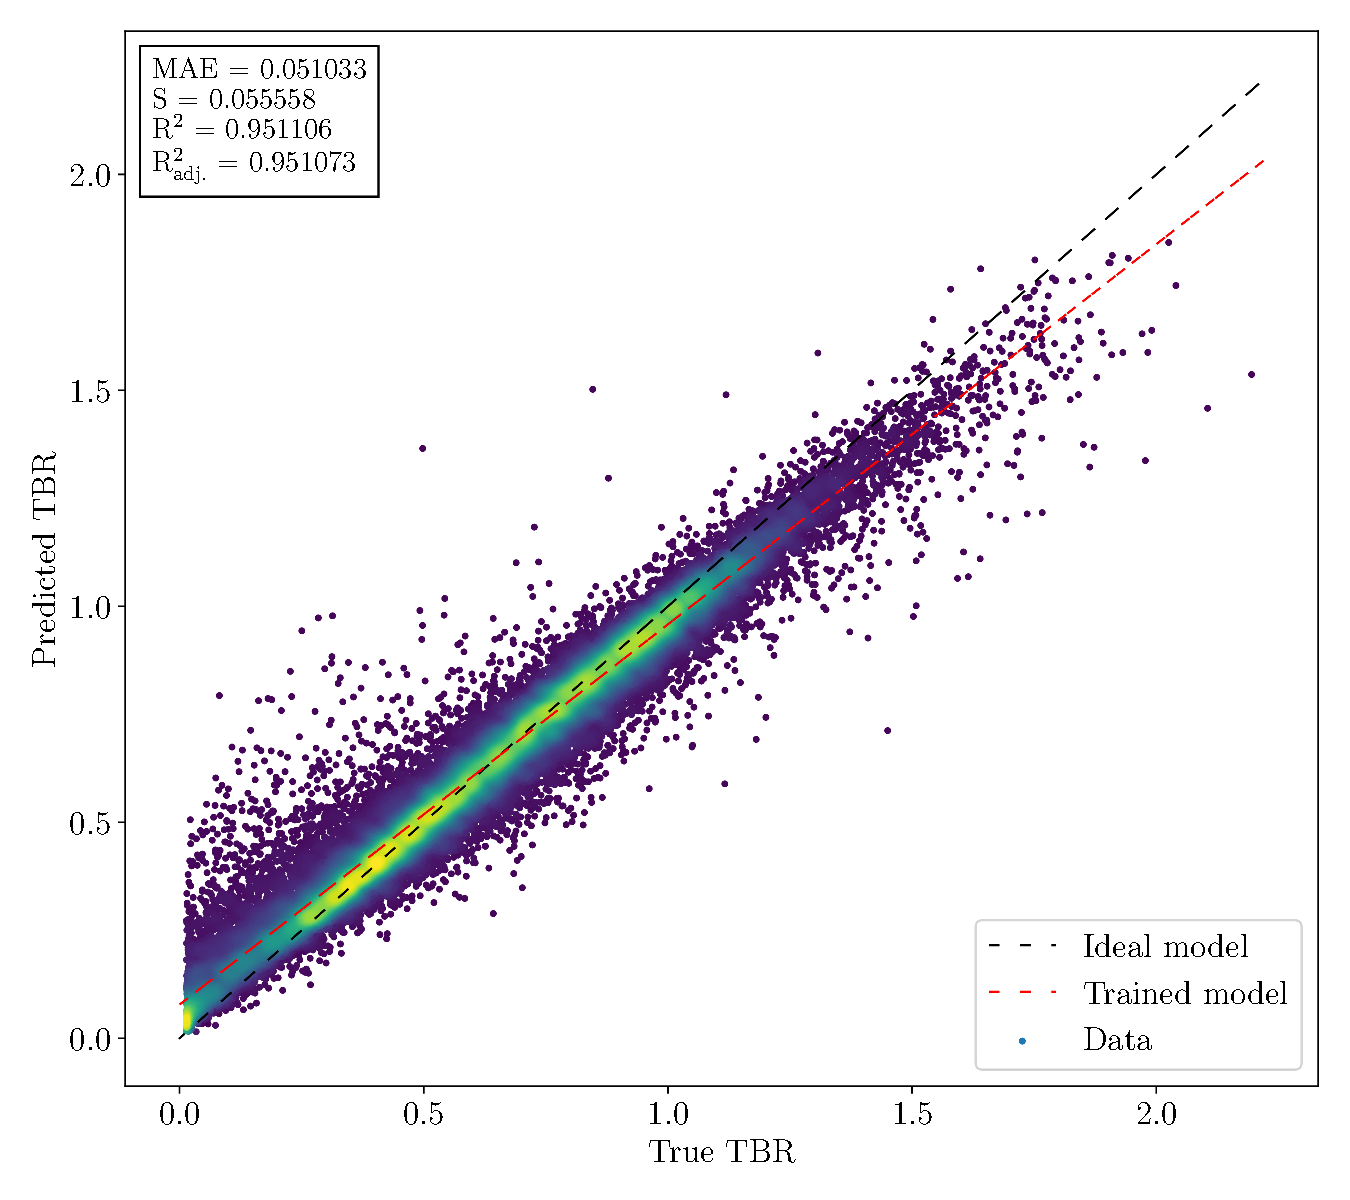
\includegraphics[height=60pt]{exp4_model4_rasterized}\hfill%
		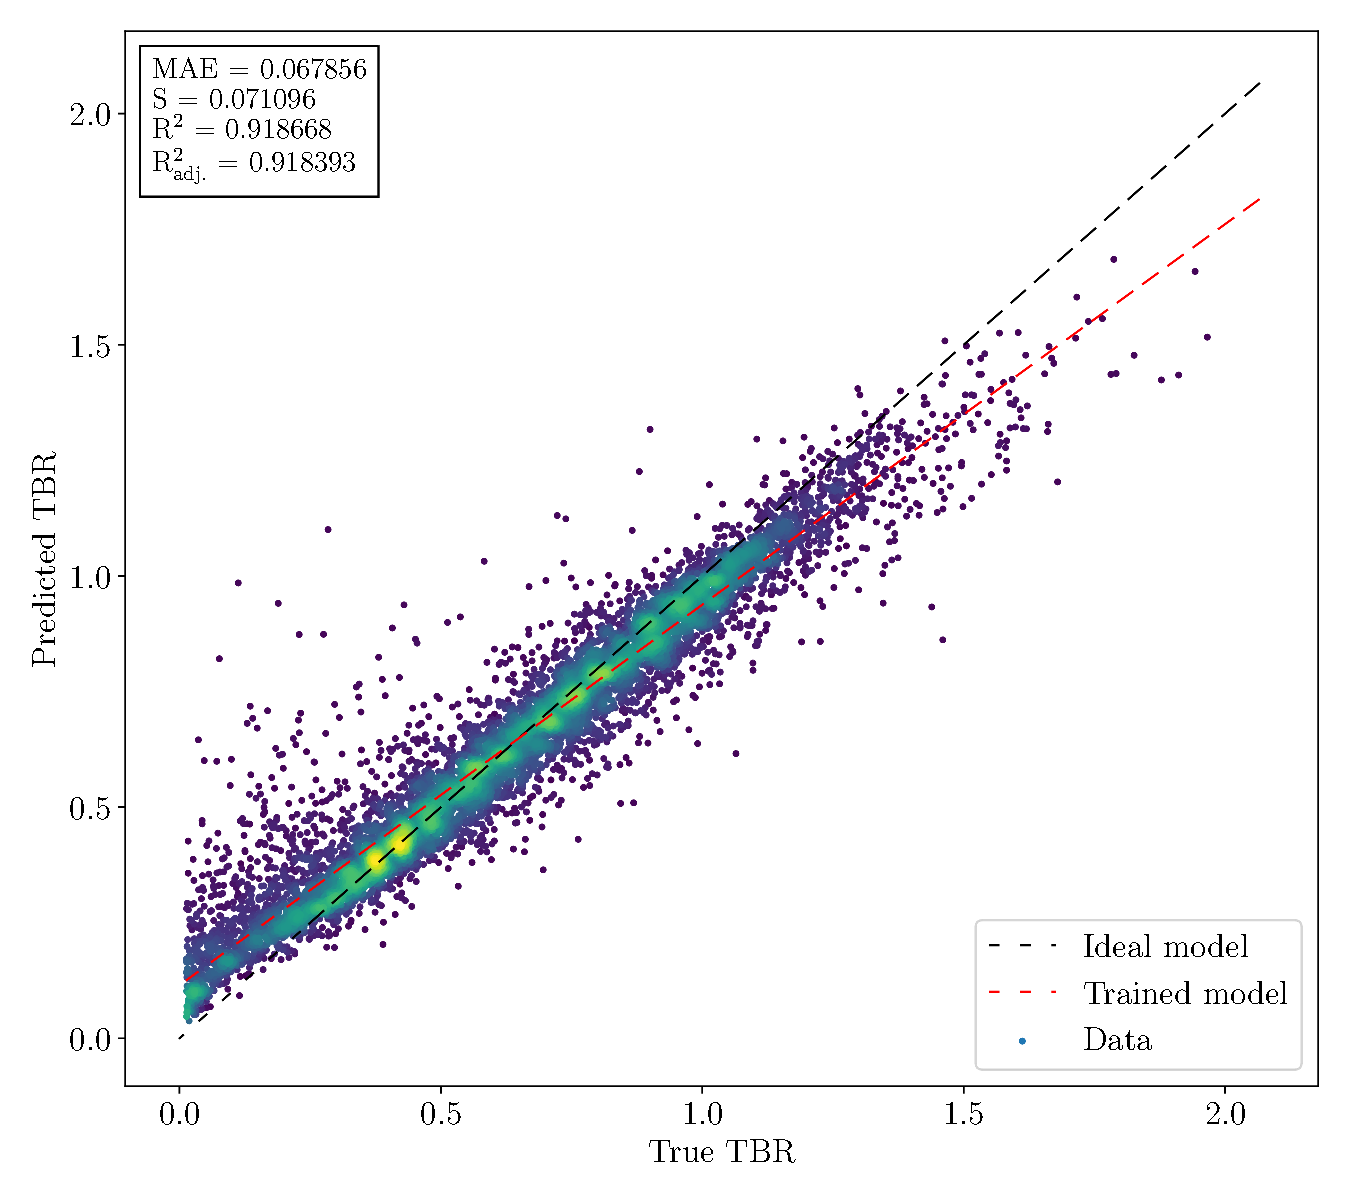
\includegraphics[height=60pt]{exp4_model5_rasterized}\\\vspace{-4pt}%
		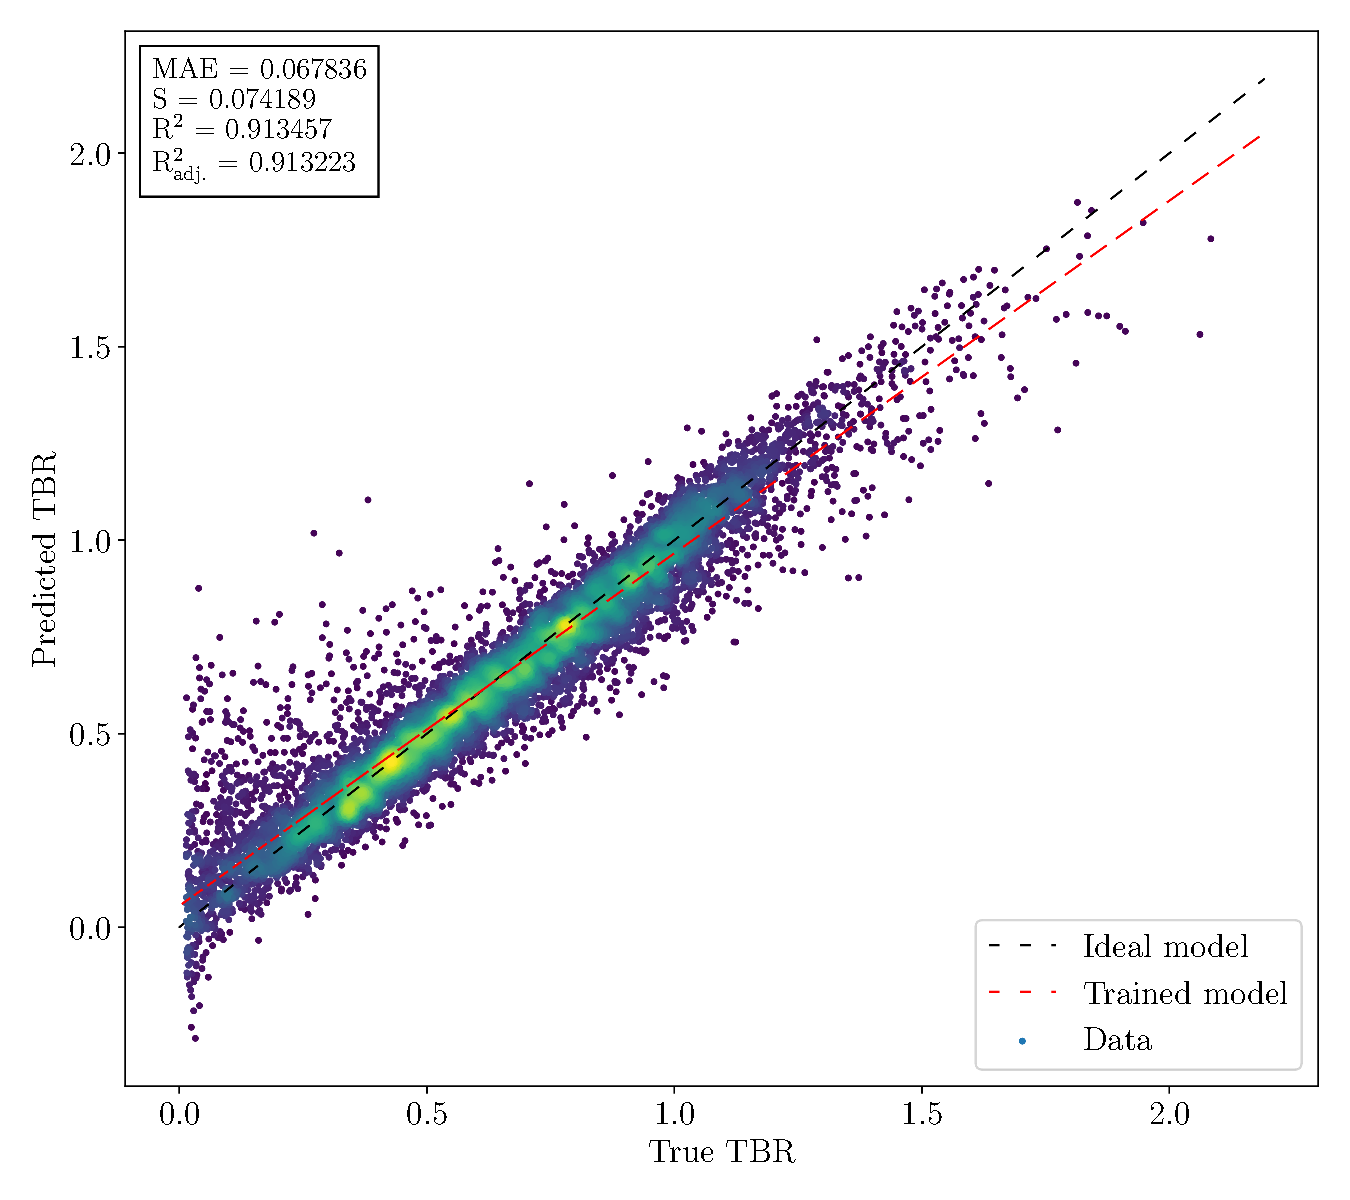
\includegraphics[height=60pt]{exp4_model2_rasterized}\hfill%
		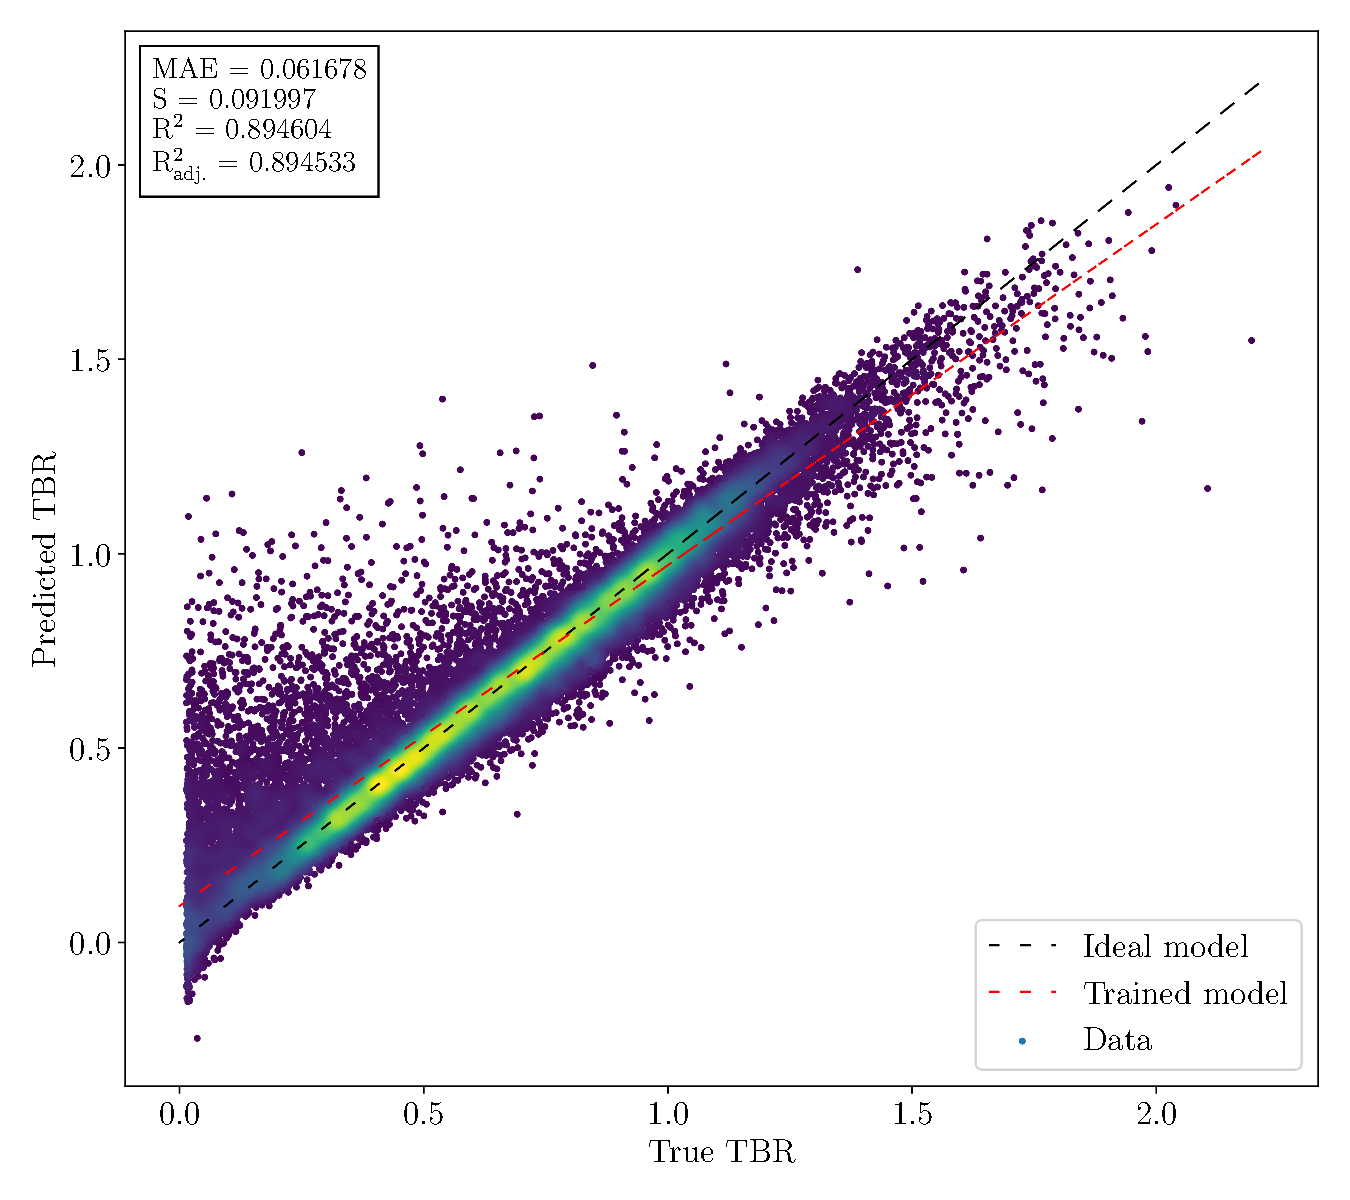
\includegraphics[height=60pt]{exp4_model8_rasterized}%
	\end{columns}
\end{frame}
